\chapter{A Grand Apparatus}\label{ch:lhc_cms}
\begin{aquote}{Fran\c{c}ois Englert, CMS: The Art of Science, 2016}
    A glance at the ATLAS and CMS detectors at CERN reveals their beauty...
    These detectors are the modern cathedrals of the rational world created by scientists, experimentalists, and theoreticians. 
\end{aquote}

\section{The Large Hadron Collider}
The Large Hadron Collider (LHC) is the largest particle accelerator ever built. 
Its most striking feature is a 27 km ring buried 175 m beneath the Franco-Swiss border (Fig.~\ref{fig:cern_aerial}) in which two beams of protons (or heavy ions like lead), after going through several smaller stages (Fig.~\ref{fig:cern_complex}), are accelerated to 99.9999991\% of the speed of light in opposite directions. 
The beams are steered by thousands of magnets, including 1232 superconducting dipole magnets, placed along the circumference of the ring. 
At various points, the proton beams are directed towards each other, allowing the protons to collide. 
These collision points are surrounded by enormous, multi-layered particle detectors which record snapshots of the collisions. 

The protons are accelerated in bunches of 115 billion, so when the bunches are brought together (called a ``bunch crossing''), over 200 billion protons are brought very close together.
However, only a small portion of them actually collide. 
During ``Run 2'' of the LHC from 2016 to 2018, for instance, there were 30 proton-proton collisions per bunch crossing on average, typically with only a single ``interesting'' collision (the ``primary vertex'') amongst them. % TODO: define pileup somehow, citation needed, plot or something of pileup needed
A collision is deemed interesting if it initiates a process that a physicist at the LHC wants to study (e.g. Fig.~\ref{fig:vbswh_feynman})---the non-interesting collisions are called ``pileup.'' 
To increase our odds of producing something truly interesting, the bunch crossings are spaced close together, with only 25 nanoseconds of separation. 
To put this into context, the speed of light is roughly 1 ft/ns, so the next bunch crossing will occur before the light from a screen on one side of the CMS control room can reach the eyes of someone standing on the other side (approximately 39 feet~\cite{CMSP5Layout}).
Therefore, particle detectors on the LHC must be capable of excellent resolution \textit{and} high throughput. 
That is, they must be able to resolve the particles from the primary vertex amongst the many others produced by the pileup, all within the 25 ns between bunch crossings. 

\begin{figure}[htb]
    \centering
    \includegraphics[width=0.95\textwidth]{fig/lhc/lhc_complex.png}
    \caption{
        The CERN complex illustrated in detail, from Ref.~\cite{Lopienska:2800984}. 
        The different stages of particle acceleration can be seen in detail, described here for protons. 
        First, negative hydrogen ions (H$^-$) generated by LINAC 4 are fed into BOOSTER, which strips the electrons from the H$^-$ ions, leaving only the protons, and accelerates them to 2\GeV. 
        Next, the Proton Synchrotron (PS) accelerates the protons to 26\GeV. 
        The PS feeds into the Super Proton Synchrotron (SPS) which further accelerates them to to 450\GeV. 
        Finally, the protons are fed into the LHC, which accelerates them to a final energy of 7\TeV. 
    }
    \label{fig:cern_complex}
\end{figure}

\begin{figure}[htb]
    \centering
    \includegraphics[width=0.9\textwidth]{fig/lhc/cern_aerial_view.jpg}
    \caption{
        The CERN complex pictured from a ``bird's eye'' view, from Ref.~\cite{Maximilien:1295244}. 
        The SPS and LHC tunnels are drawn on top of the landscape in light blue and yellow, respectively, and the Franco-Swiss border is drawn as a dashed white line. 
    }
    \label{fig:cern_aerial}
\end{figure}

\section{The Compact Muon Solenoid}
The Compact Muon Solenoid (CMS) Experiment is one of two general purpose LHC experiments, the other being the ATLAS\footnotemark{} Experiment, among the four major experiments supported by the LHC~\cite{LHCWeb}, where the other two are more specialized: ALICE, for studying heavy ion collisons, and LHCb, for studying b quarks. 
\footnotetext{Where ATLAS is, putting it politely, a rather creative acronym: ``A Toroidal LHC ApparatuS.''}
Compared to ATLAS, which stands at a mighty $46\times25\times25$ meters in dimension, CMS is ``compact'' at a stout $21\times15\times15$ m, with a dedicated muon system and one of the world's largest solenoid magnets~\cite{ATLASWeb, CMSWeb}. 
See Fig.~\ref{fig:cms_labeled} for its exact specifications, and Figures~\ref{fig:cms_pics} and \ref{fig:cms_jguiang} for some beauty shots. 

CMS is composed of subdetectors arranged in concentric layers, where each layer interacts with, or completely absorbs, certain particles, producing an electric signal that can be used to infer some property of those particles. 
The innermost layer is the silicon tracker, which allows for the reconstruction of the trajectory of throughgoing charged particles. 
Next is the electromagnetic calorimeter (ECAL), which absorbs electrons and photons and records their individual energies. 
After the ECAL, there is the hadronic calorimeter (HCAL), which instead absorbs hadrons and records their individual energies. 
These first three layers---the tracker, ECAL, and HCAL---are surrounded by the superconducting solenoid, which immerses them in an approximately uniform magnetic field that runs parallel to the beamline. 
This is critical: because charged particles fly along curved trajectories in a magentic field according to their charge and momentum, those properties can be inferred from a high-quality measurement of each particle's trajectory. 
Finally, there are alternating layers of muon chambers and iron support structures. 
The former detects throughgoing muons, which pass through all of the inner layers mostly unperturbed, while the latter conveniently helps absorb any stray particles that should have been absorbed by the ECAL or HCAL. 
In a perfect world, where the detector is 100\% efficient, the exact identity of any individual particle can be inferred based on which detectors registered a signal (Fig.~\ref{fig:cms_particle_id}). 
For example, a photon only leaves a deposit in the ECAL, while a charged hadron leaves behind ``hits'' in the tracker as well as a deposit in the HCAL. 
The exact function of each subdetector layer described here is detailed below.

\begin{figure}[htb]
    \centering
    \includegraphics[width=0.9\textwidth]{fig/cms/cms_labeled.jpg}
    \caption{
        Lorem ipsum.
    }
    \label{fig:cms_labeled}
\end{figure}

\begin{figure}[htb]
    \centering
    \subfloat{\includegraphics[width=0.465\textwidth]{fig/cms/particle_id_sandwich.png}}\quad
    \subfloat{\includegraphics[width=0.435\textwidth]{fig/cms/cms_slice.png}}
    \caption{
        A generic, general-purpose particle detector (left) and CMS (right), showing the signals left by different kinds of particles.
    }
    \label{fig:cms_particle_id}
\end{figure}

\subsection{Superconducting solenoid}
\subsection{Silicon tracker}
\subsection{Electromagnetic calorimeter}
\subsection{Hadronic calorimeter}
\subsection{Muon chambers}

\begin{figure}[htb]
    \centering
    \subfloat{\includegraphics[width=0.465\textwidth]{fig/cms/cms_picture1.jpg}}\quad
    \subfloat{\includegraphics[width=0.435\textwidth]{fig/cms/cms_picture2.jpg}}
    \caption{
        The Compact Muon Solenoid in all of its glory, with one of the endcaps separated from the main body of the experiment, pictured from the top (left) and side (right). 
    }
    \label{fig:cms_pics}
\end{figure}

\begin{figure}[htb]
    \centering
    \subfloat{\includegraphics[width=0.482\textwidth]{fig/cms/cms_picture3.jpg}}\quad
    \subfloat{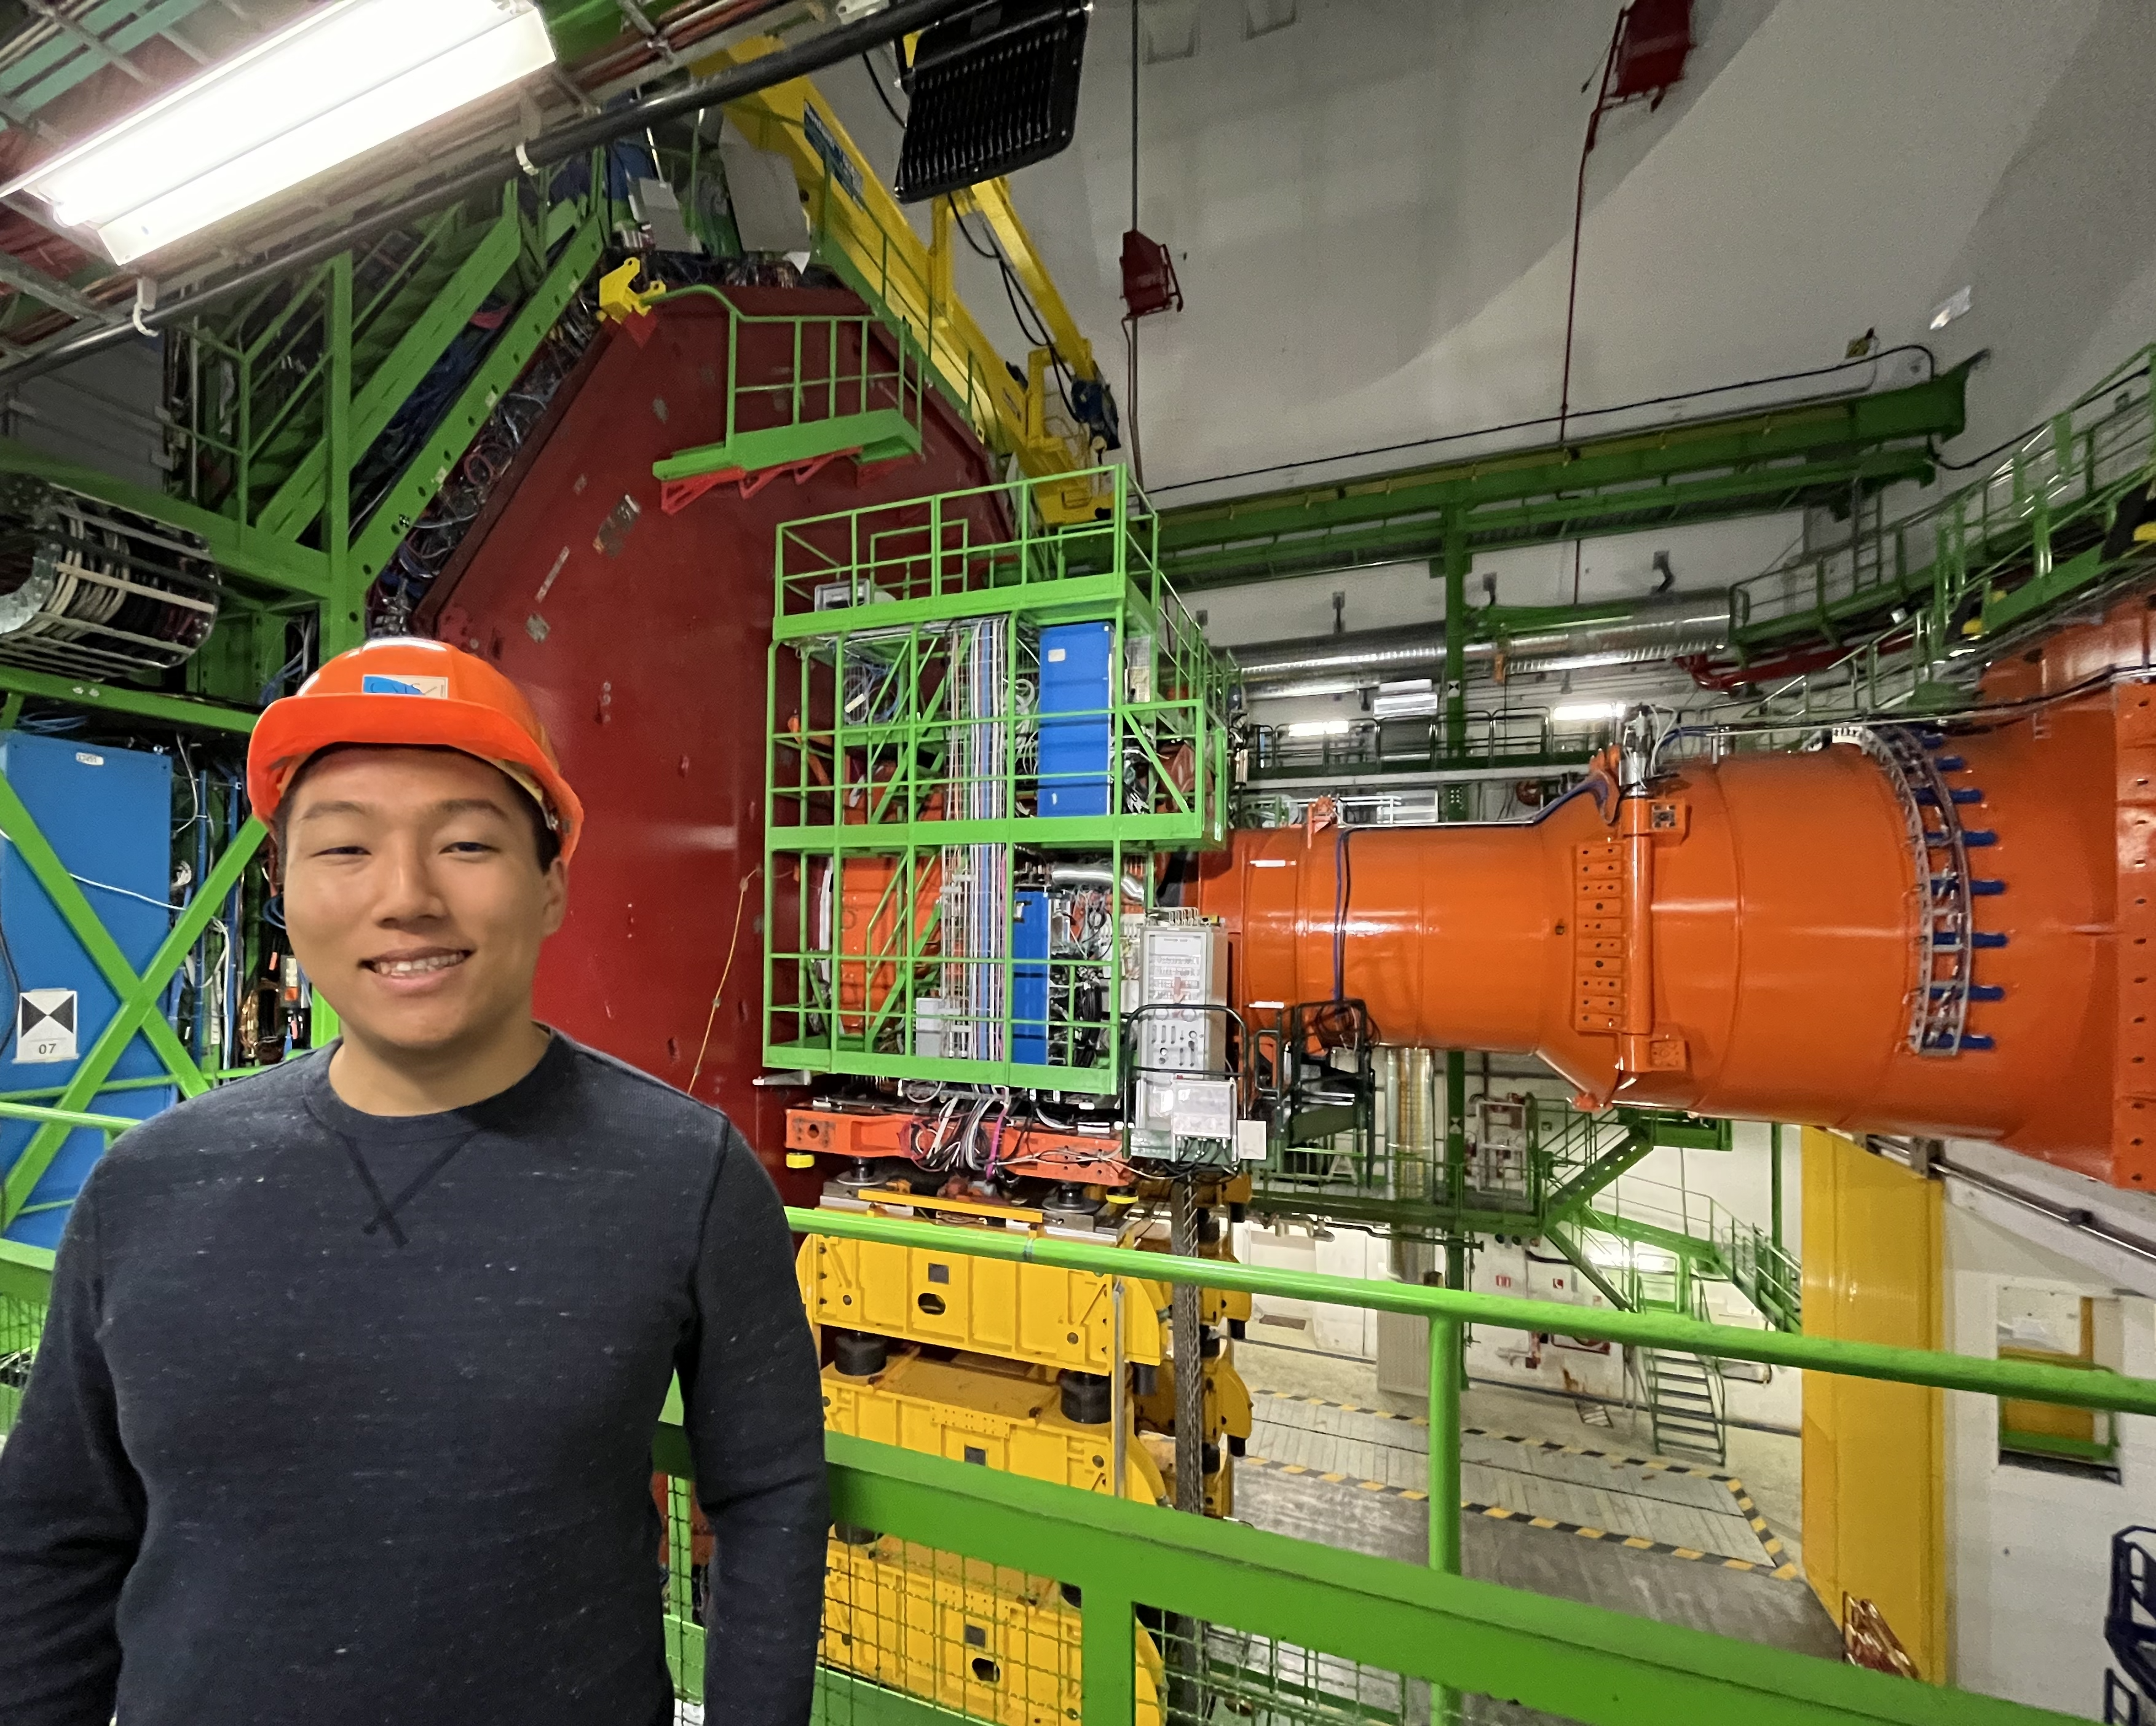
\includegraphics[width=0.4\textwidth]{fig/cms/cms_jguiang.jpg}}
    \caption{
        The Compact Muon Solenoid in the closed configuration, pictured from the top (left) and side, with a physicist in the foreground for scale (right).
    }
    \label{fig:cms_jguiang}
\end{figure}

\section{The high lumonisity era}
% What is HL?
%    - show pileup plots, maybe side AND 3D volume
% What benefits does it bring?
%    - Find some papers...
% What challenges does it bring?
%    - Show CPU/Data volume plots
